\section{Introduction}\label{sec:intro}
%\begin{itemize}
%	\item Generally introduce dialog acts
%	\item Need for automated tagging
%	\item Current SotA
%	\item Introduce distributional representations
%	\item Present hypotheses
%	\item ...
%	\item Set up rest of report
%\end{itemize}
Discourse structure analysis is fundamental for understanding spontaneous dialogs and developing human-computer dialog systems.
An essential part of discourse structure analysis is the identification of dialog act classes (e.\ g.\ \emph{questions}, \emph{self-talks}, \emph{statements}, \emph{backchannels}).
As defined by Austin \lau{add citation}, dialog acts present linguistic abstractions of the illocutionary force of speech acts and model the communicative intention in an utterance in a conversation. There are several tasks that have dialog acts as an input for their computations. Examples of these include speech recognition, speech synthesis, summarization, and of course, human-machine dialog systems. As a result, correctly identifying dialog act tags is fundamental for such tasks.


Table~\ref{tab:swda_example} shows an example of dialog acts from the Switchboard corpus we are trying to classify.

\begin{table}[h]
\centering
\begin{tabular}{c l l}
\hline
\textbf{Speaker} & \textbf{Tag} & \textbf{Utterance}
\\
\hline
B & Wh-Question & how old is your daughter?\\
A & Statement-non-opinion & she's three.\\
B & Summarize & oh , so she's a little one.\\
A & Agree & yes.\\
B & Acknowledge & yeah.\\
A & Statement-non-opinion & she's, she's little.\\
\hline
\end{tabular}
\caption{SWDA dialog excerpt.}
\label{tab:swda_example}
\end{table}

For the purpose of this work, we extract feature representations for entire utterances in an unsupervised fashion.
For that we build a distributional semantic model that learns vector representations for entire utterances and then use these vector features as inputs for different machine learning classifiers.
Several techniques can be used for mapping text units to a high dimensional real value space.
Utterance embeddings have the attractive property of representing an entire textual sequence as a vector while taking word order into account, as opposed to the classical \emph{Bag-of-words} approach in which word order is not preserved and in which resulting vectors show no semantic relations.
We expect this encapsulated extra information to play an important role in the classification task. In order to infer those embeddings we use the \emph{paragraph2vec} framework recently introduced by \cite{le2014distributed}, which is based on the previous word embedding models by \cite{mikolov2013efficient}.

\roger{I would put the following two paragraphs about embeddings into 3.1 Utterance Embeddings}
Neural networks for semantics has gained relevant importance in the past years, since the publication of the first neural networks word embedding models. One of the main reasons for this to happen, is the fact that the resulting vector representations are able to effectively capture the meaning of words given their context. Figure~\ref{fig:w2v_example} shows a typical example of this characteristic.

\begin{figure}
\centering
\begin{minipage}{.4\textwidth}
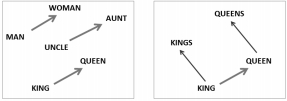
\includegraphics[width=1\textwidth]{img/w2v_example}
\caption{Word2vec semantic relations.}
\label{fig:w2v_example}
\end{minipage}
\end{figure}

In these models, word embeddings are learned by predicting words within a context (depending on the neural network model -i.e. CBOW or Skip-gram, it could be that the network tries to predict a word given a context, or the context given a word), due to the co-occurrence of words in texts, given the use of a language, these models are capable of successfully coming up with mathematical representations of words. This idea of word co-occurrences is not longer valid when we take sentences as units; a sentence can have -potentially- any other valid sentence before and after. Instead, a neural network for learning representations for sentences has been proposed, in which the sentence structures are learned from the words that are included in it. \lau{add cite} In this case, word embeddings and sentence embeddings are trained simultaneously, as a sentence vector, shared across the words within the phrase, is maintained and updated in parallel to the word vectors.  This unsupervised model makes it possible to map sentences (utterances) of any length to vectors of fixed length. Moreover, an interesting characteristic of this model is that multiple corpora can be used as input for training, allowing us to create huge training sets, based on several dialog corpora from different domains and characteristics.

For the actual dialog act tagging we treat the problem as a multi-class classification task and classify utterances both in isolation as well as in the context of the previous utterances. We evaluate the tagging accuracy and compare different models. Besides the baselines set up by previous work, we compare the results against a simple baseline that uses a bag-of-words (BOW) representation for each utterance. 

The outline of this report is set as follows: in Section 2, we present relevant approaches that aim at classifying dialog acts and briefly describe their main characteristics and results. In Section 3, we specify the datasets used in our experiments, present the model to infer utterance embeddings and we detail the properties of our classification pipeline. An exhaustive analysis of the results of the experiments is presented in Section 4. Finally, Section 5 includes conclusions drawn from this work as well as issues and future work. \lau{check}